\documentclass[times, utf8, zavrsni, numeric]{fer}
\usepackage{booktabs}
\usepackage[hidelinks]{hyperref}
\usepackage{graphicx}
\usepackage{bm}

\setlength\parindent{24pt}
\newcommand{\matr}[1]{\mathbf{#1}}
\newcommand{\hiperravnina}{$\langle \mathbf{w}, b \rangle$}

\interfootnotelinepenalty=10000

\graphicspath{{"D:/fer/6. semestar/ZAVRAD/svm-sentiment-analysis/Thesis/Slike/"}}

\begin{document}

% TODO: Navedite broj rada.
\thesisnumber{5179}

% TODO: Navedite naslov rada.
\title{Primjena stroja s potpornim vektorima za analizu sentimenta korisničkih recenzija}

% TODO: Navedite svoje ime i prezime.
\author{Dominik Stanojević}

\maketitle

% Ispis stranice s napomenom o umetanju izvornika rada. Uklonite naredbu \izvornik ako želite izbaciti tu stranicu.
\izvornik

% Dodavanje zahvale ili prazne stranice. Ako ne želite dodati zahvalu, naredbu ostavite radi prazne stranice.
\zahvala{Hvala Kurtzu.}

\tableofcontents

\chapter{Uvod}

\par Klasifikacijski i regresijski problemi jedni su od najvažnijih problema strojnog učenja. 
Modeli poput linearne i logističke regresije pogodni su za jednostavnije probleme.
Zahvaljujući sve većoj dostupnosti podataka i povećanju procesorske moći današnjih računala,
pojavljuju se složeniji zadaci za koje navedene metode nisu efikasne.

\par Pojava složenijih zadataka rezultirala je i pojavom složenijih metoda koje mogu doskočiti 
istima. Modeli poput slučajnih šuma i modeli iz skupine dubokog učenja u mogućnosti su rješavati i složenije, 
nelinearne proble me.

\par Osim navedenih modela, još jedan model koji je sposoban efikasno obraditi nelinearne podatke 
je \textbf{stroj s potpornim vektorima} (engl. \textit{Support Vector Machine}, u nastavku SVM).
Koristeći jezgreni trik, stroj s potpornim vektorima uspješno razdvaja linearno nerazdvojive podatke.
Iako su temeljne ideje modela predstavljene prije više od pola stoljeća, stroj s potpornim vektorima i danas je jedan od
najrobusnijih modela za klasifikaciju i regresiju.

\par Jedan od zanimljivih problema koji dobro prikazuje robusnost SVM-a je \textbf{analiza sentimenta}
(engl. \textit{Sentiment Analysis}).
Subjektivnost emocija, kontekst te velika količina podataka svakako predstavljaju izazove u rješavanju problema.
Koristeći SVM, uz uvjet kvalitetnog pretprocesiranja podataka, mogu se postići zavidni rezultati u polju analize sentimenta.

\par U radu je predstavljen model stroja s potpornim vektorima te problem analize sentimenta.
U poglavlju \ref{ppodrucja} bit će predstavljen pregled područja, povijest modela stroja s potpornim vektorima te problem analize sentimenta.
U poglavlju \ref{svm} detaljnije će se obraditi model SVM.
Bit će opisana motivacija i interpretacija modela.
Nadalje, detaljnije će se pojasniti algoritmi optimizacije modela.
U poglavlju \ref{sentiment} formalizirat će se problem analize sentimenta.
Prikazat će se postupak pretprocesiranja podataka koji će podatke pretvoriti u oblik razumljiv SVM-u.
U petom poglavlju, provest će se eksperiment analize korisničkih recenzija uporabom opisanih metoda.
Ukratko će se analizirati dobiveni rezultati.
Poglavlje \ref{zakljucak} sadrži zaključak i ideje za daljnje istraživanje. 

\chapter{Pregled područja} \label{ppodrucja}
Započinje \cite{vapnik1963}

\chapter{Stroj s potpornim vektorima} \label{svm}
U ovom poglavlju bit će predstavljen model stroja s potpornim vektorima. 
Potpoglavlje \ref{klasifikacija} definira pojam klasifikacije i pojašnjava razliku između klasifikacije i regresije.
U potpoglavlju \ref{hmargine} pojasnit će se ideja razdvajajuće hiperravnine.
Potpogljavlje \ref{margina} predstavit će pojam margine razdvajajuće hiperravnine i njenu važnost u izgradnji
klasifikatora.
Koristeći ideje iz prethodnih potpoglavlja, potpoglavlje \ref{opthiper} definira optimalnu razdvajajuću hiperravninu,
metodu koju koristi SVM prilikom klasifikacije podataka.
Potpoglavlje \ref{jezgra} opisuje transformaciju prostora značajki koristeći jezgrene trikove.
Jezgreni trikovi su efikasne metode koje omogućuju razdvajanje originalno linearno nerazdvojivih podataka.
U potpoglavlju \ref{reg} daje se ideja regularizacije. Ova metoda omogućuje da stroj s potpornim vektorima
pronađe optimalnu hiperravninu u slučaju linearno nerazdvojivih podataka.

\section{Klasifikacija} \label{klasifikacija}
Problemi nadziranog učenja uobičajno se dijele na dvije podskupine - klasifikaciju i regresiju.
Neka vektorski prostor $\textit{X}$ dimenzije $n$, primjerice $\mathbb{R}^n$, predstavlja skup primjeraka. 
Pojedini primjerak može se zadati vektorom: $\mathbf{x}=(x_1,x_2,\dots,x_n)$.
Ako pojedinom primjerku $\mathbf{x}$ pridružimo oznaku razreda $y$, tada se govori o \textbf{klasifikaciji}.
Pojednostavljeno, postupkom klasifikacije određuje se razred kojoj određen primjerak $\mathbf{x}$ pripada.
Skup svih razreda $\textit{C}$ je konačan, a broj razreda dan je kardinalitetom $\left\vert{C}\right\vert$.

\begin{figure}
\centering
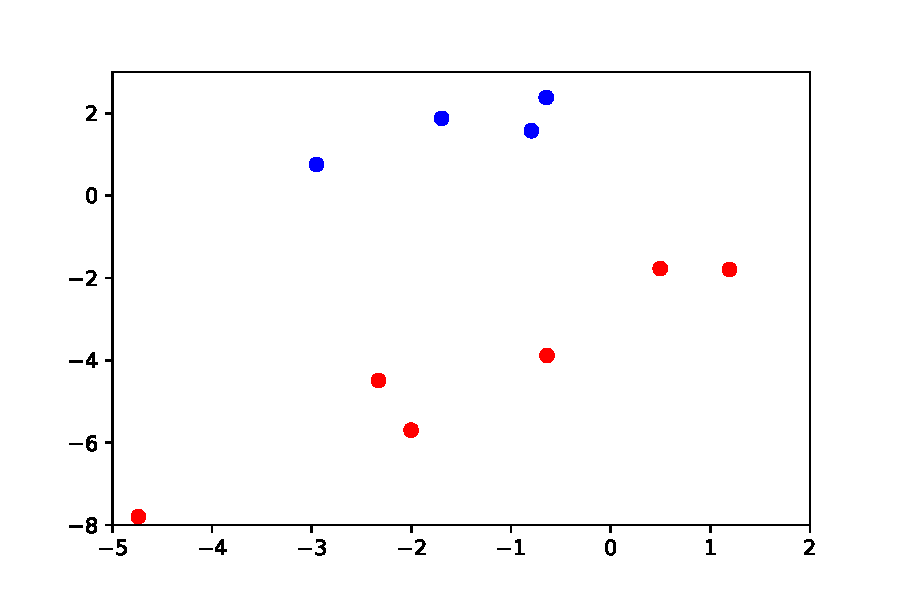
\includegraphics{klas.pdf}
\caption{Primjer klasifikacijskog problema}
\label{fig:klas}
\end{figure}


\par Primjer klasifikacijskog problema prikazan je slikom \ref{fig:klas}. 
Prostor primjeraka je $\mathbb{R}^2$, a skup razreda je dvočlani skup tj. $\left\vert{C}\right\vert=2$.
Klasifikacija podataka u dvočlane skupove naziva se \textbf{binarna klasifikacija}.
Upravo je stroj s potpornim vektorima primjer binarnog klasifikatora, no postoje metode koje pružaju mogućnost
višerazredne klasifikacije.
Osim gore navedenog primjera, još neki primjeri klasifikacije su okrivanje neželjene pošte, prepoznavanje rukopisa,
prepoznavanje prometnih znakova, itd..

\par Za razliku od problema klasifikacije u kojem je varijabli $y$ pridružena vrijednost iz konačnog skupa, 
kod problema regresije primjerku pridružujemo vrijednost iz nekog beskonačnog skupa, primjerice $\mathbb{R}$.
Postoji modifikacija stroja s potpornim vektorima koji omogućuje rješavanje regresijskih problema.
Primjeri regresije su izračun plaće u ovisnosti o spolu, obrazovanju i sl., određivanje postotka glasova
kandidata na izborima, itd.

\section{Razdvajajuća hiperravnina} \label{hmargine}
Interpretaciju modela stroja s potpornim vektorima potrebno je započeti s pojmom koji nije strogo vezan uz sam model.
Primjerice model logističke regresije, iako temeljen na vjerojatnosti, u konačnici pronalazi hiperravninu kojom razdvaja
podatke.

\par Neka je zadan vektorski prostor $\textit{X}$ dimenzije $n$, primjerice $\mathbb{R}^n$.
Tada je \textbf{hiperravnina} definirana kao potprostor dimenzije $n-1$ unutar prostora $\textit{X}$.
Primjerice, u jednodimenzijskom prostoru hiperravnina je točka, u dvodimenzijskom prostoru
 hiperravninu predstavlja bilo koji pravac koji leži u ravnini, a u trodimenzijskom prostoru hiperravnina
 je predstavljena ravninom. 
Analogno, pojam hiperravnine vrijedi i za prostore većih dimenzija. 

\par Za hiperravninu zadanom jednadžbom $f(\mathbf{x})=b + \mathbf{w}^T\mathbf{x} = 0$ 
vrijede sljedeća svojstva:
\begin{enumerate}
  \item za svaku točku $T$ na hiperravnini vrijedi: $b = -\mathbf{w}^T\mathbf{x}$,
  \item jedinični vektor normale je zadan izrazom: $\mathbf{n} = \frac{\mathbf{w}}{\|\mathbf{w}\|}$,
  \item udaljenost točke $P$ od hiperravnine iznosi: $d = \frac{f(\mathbf{x})}{\|\mathbf{w}\|}$.
\end{enumerate}

Hiperravnina ovisi o vektoru težina $\mathbf{w}$ i slobodnom članu $b$. 
U daljnjem tekstu hiperravnina bit će zadana svojim parametrima, \hiperravnina{}. 

\par Hiperravnine same po sebi nisu pretjerano interesantne. 
No, za klasifikaciju interesantan je određen podskup hiperravnina.
Hiperravnina koja razdvaja dva razreda podataka naziva se \textbf{razdvajajuća hiperravnina.}
Uz pretpostavku $y \in \{-1, 1\}$, za razdvajajuću hiperravninu vrijedi:
\begin{equation}
  y^{(i)} = sgn(b + \mathbf{w}^T\mathbf{x}^{(i)}), \forall i
\end{equation}
gdje je $\mathbf{x}^{(i)}$ primjer iz skupa podataka, a $y^{(i)}$ je oznaka razreda pridružena primjeru $\mathbf{x}^{(i)}$.

\begin{figure}
\centering
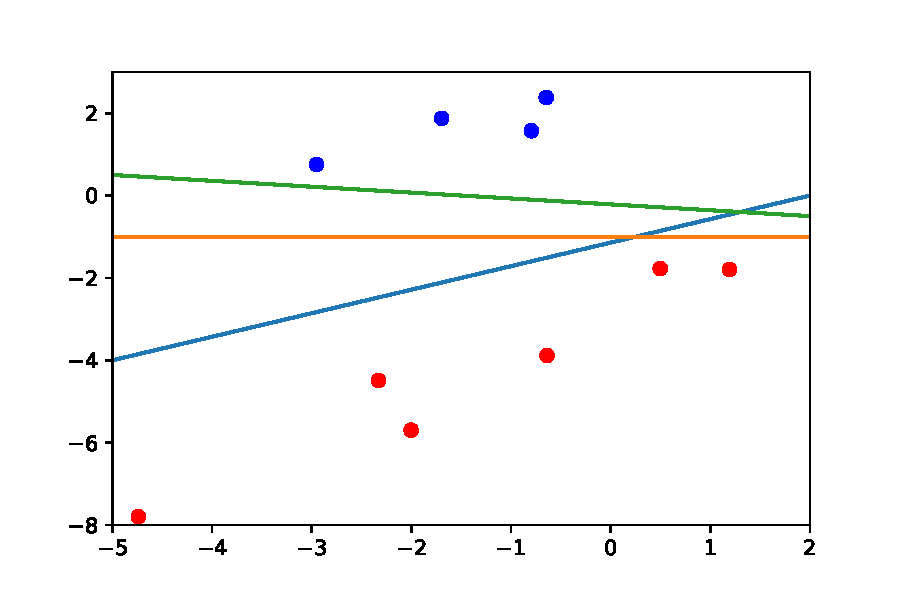
\includegraphics{hravnine.pdf}
\caption{Razdvajajuće hiperravnine}
\label{fig:hrav}
\end{figure}

Na slici \ref{fig:hrav} prikazani su primjerci jednaki onima sa slike \ref{fig:klas}.
Također, prikazane su i tri razdvajajuće hiperravnine. 
Valja primijetiti kako je moguće konstruirati beskonačno mnogo razdvajajućih hiperravnina.

\section{Margina razdvajajuće hiperravnine} \label{margina}
Za razliku od drugih klasifikatora koji traže bilo koju razdvajajuću hiperravninu kako bi klasificirali podatke,
stroj s potpornim vektorima uzima u obzir i udaljenosti primjeraka od hiperravnine. 
Intuitivno se može zaključiti kako je sigurnije odrediti razred za one primjerke koji su udaljeniji od 
hiperravnine. Udaljenost primjerka od hiperravnine nazivamo \textbf{margina}.

\par Neka je zadan $i$-ti primjerak $(\mathbf{x}^{(i)}, y^{(i)})$ gdje je $\mathbf{x}^{(i)}$ vektor značajki, 
a $y^{(i)}$ pripadajuća oznaka razreda.
Također, neka je $\mathbf{r^{(i)}}$ radij-vektor točke $T$ koja se nalazi na hiperravnini i najmanje je udaljena od primjerka. 
Udaljenost $i$-tog primjerka od hiperravnine iznosi $m^{(i)}$. 
Vrijede dvije jednadžbe:
$$\mathbf{r}^{(i)} = \mathbf{x}^{(i)} - y^{(i)}m^{(i)}\frac{\mathbf{w}}{\|\mathbf{w}\|},$$
$$b + \mathbf{w}^T\mathbf{r^{(i)}} = 0.$$
Riješavanjem ovog sustava po $m^{(i)}$ dobiva se margina hiperravnine \hiperravnina{}
s obzirom na primjerak $(\mathbf{x}^{(i)}, y^{(i)})$:
\begin{equation}
  m^{(i)} = \frac{y^{(i)}(b + \mathbf{w}^T\mathbf{x}^{(i)})}{\|\mathbf{w}\|}.
  \label{eq:marg}
\end{equation}

\begin{figure}
\centering
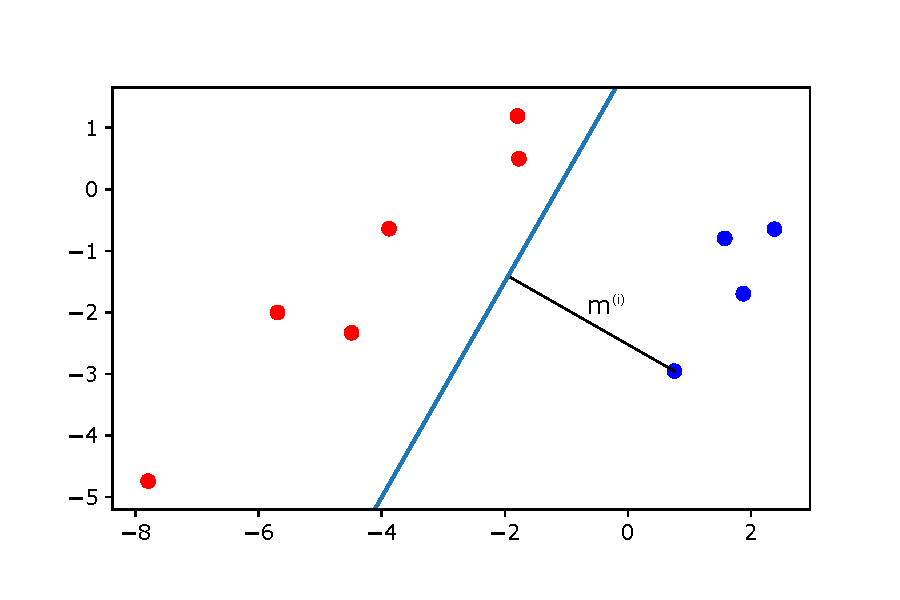
\includegraphics{distance.pdf}
\caption{Margina hiperravnine s obzirom na primjerak $(\mathbf{x}^{(i)}, y^{(i)})$}
\label{fig:mex}
\end{figure}

\par Na slici \ref{fig:mex} prikazana je udaljenost primjerka od razdvajajuće hiperravnine.
Valja uočiti kako za pozitivne oznake razreda, $y^{(i)} = 1$, vrijednost $b + \mathbf{w}^T\mathbf{x}^{(i)}$ je pozitivna.
Analogno, za $y^{(i)} = -1$ vrijednost $b + \mathbf{w}^T\mathbf{x}^{(i)}$ je negativna.
Može se zaključiti kako je vrijednost margine za svaki primjerak strogo pozitivna. 
U slučaju hiperravnine koja ne razdvaja podatke to svojstvo ne vrijedi.

\par Osim svojstva pozitivnosti, za marginu je zanimljiva i otpornost na skaliranje. 
Neka je hiperravnina \hiperravnina{} skalirana nekim faktorom $k$. Za marginu $m^{'(i)}$ vrijedi:
\begin{equation*}
  m^{'(i)} = \frac{y^{(i)}(kb + k\mathbf{w}^T\mathbf{x}^{(i)})}{\|k\mathbf{w}\|} =
  \frac{y^{(i)}k(b + \mathbf{w}^T\mathbf{x}^{(i)})}{k\|\mathbf{w}\|} = m^{(i)}.
\end{equation*}
Ovo svojstvo omogućuje da duljina vektora težina bude proizvoljna što će se pokazati veoma korisnim kod
postavljanja optimizacijskog problema.

\par Nakon definiranja margine hiperravnine za pojedini primjerak, potrebno je definirati 
i marginu hiperravnine uzimajući u obzir cijeli skup podataka za učenje. 
\textbf{Margina hiperravnine} u odnosu na skup podataka za učenje 
je margina onog primjerka koji je najbliži hiperravnini tj.
$$M=\min_{i}m^{(i)}.$$

\section{Optimalna razdvajajuća hiperravnina} \label{opthiper}
Nakon definicije margine, sljedeći cilj je pronaći razdvajajuću hiperravninu koja najbolje razdvaja podatke.
Uzimajući u obzir činjenicu da veća udaljenost primjerka od hiperravnine pruža veću sigurnost za ispravnu
klasifikaciju, intuitivno se može zaključiti kako će optimalna razdvajajuća hiperravnina biti ona koja
maksimizira marginu hiperravnine s obzirom na skup primjeraka za učenje. 
\textbf{Optimalna razdvajajuća hiperravnina} zadana je sljedećim optimizacijskim problemom:

\begin{equation}
\begin{aligned}
& \underset{\mathbf{w}, b}{\text{max}}
& & M \\
& \text{s obzirom na}
& & y^{(i)}(\mathbf{w}^T\mathbf{x}^{(i)} + b) \geq M, \; i = 1, \ldots, N \\
&&& \|\mathbf{w}\|=1.
\end{aligned}
\end{equation}

\par Gledajući gornji problem, može se uočiti kako su uvedena dva ograničenja. 
Ova ograničenja omogućuju da su svi primjerci udaljeni od hiperravnine za minimalno $M$.
Drugo ograničenje koje normalizira vektor težina onemogućuje rješavanje problema u ovom obliku budući da
uvjet $\|\mathbf{w}\|=1$ nije konveksan. Koristeći jednadžbu \ref{eq:marg}, oba ograničenja mogu se svesti
na jedno: 
\begin{equation*}
  y^{(i)}(\mathbf{w}^T\mathbf{x}^{(i)} + b) \geq M\|\mathbf{w}\|, \; i = 1, \ldots, N.
\end{equation*}

Nadalje, budući da duljina vektora težina ne utječe na marginu i klasifikaciju, moguće je proizvoljno odabrati
njegovu duljinu.
Za $\|\mathbf{w}\|=\frac{1}{M}$ cilj optimizacije se svodi na pronalazak maksimuma funkcije 
$f(\mathbf{w}) = \frac{1}{\|\mathbf{w}\|}$. Znajući kako se maksimizacija ove funkcije može svesti na 
minimizaciju kvadrata norme, može se pisati:

\begin{equation}
\begin{aligned}
& \underset{\mathbf{w}, b}{\text{min}}
& & \frac{1}{2}\|\mathbf{w}\|^2 \\
& \text{s obzirom na}
& & y^{(i)}(\mathbf{w}^T\mathbf{x}^{(i)} + b) \geq 1, \; i = 1, \ldots, N.
\end{aligned}
\end{equation}

\par Koristeći nekoliko različitih transformacija, problem je redefiniran na jednostavniji način.
Budući da je dobivena konveksna kvadratna funckija cilja uz linearne uvjete ovaj problem je rješiv
metodama kvadratnog programiranja. Kasnije u radu će se ovaj optimizacijski problem dodatno transformirati
kako bi se iskoristili algoritmi koji rješavaju problem efikasnije od generičkog softvera za 
rješavanje ovakvih optimizacijskih problema. 

\section{Regularizacija} \label{reg}
U dosadašnjem radu klasificiralo se linearno razdvojive podatke. 
Međutim, podaci najčešće nisu linearno razdvojivi ili optimalna razdvajajuća hiperravnina nije najbolji
klasifikator budući da nije otporna na stršeće vrijednosti.
Slučaj kada stršeća vrijednost utječe na izbor hiperravnine prikazan je na slici \ref{fig:outlier}.
Vidljivo je kako hiperravnina nacrtana plavom bojom dobro razdvaja podatke osim stršeće vrijednosti 
označene točkom $T$. Druga hiperravnina označena crnom bojom, iako je razdvajajuća, nije 
najsretniji izbor za klasifikaciju.

\begin{figure}
\centering
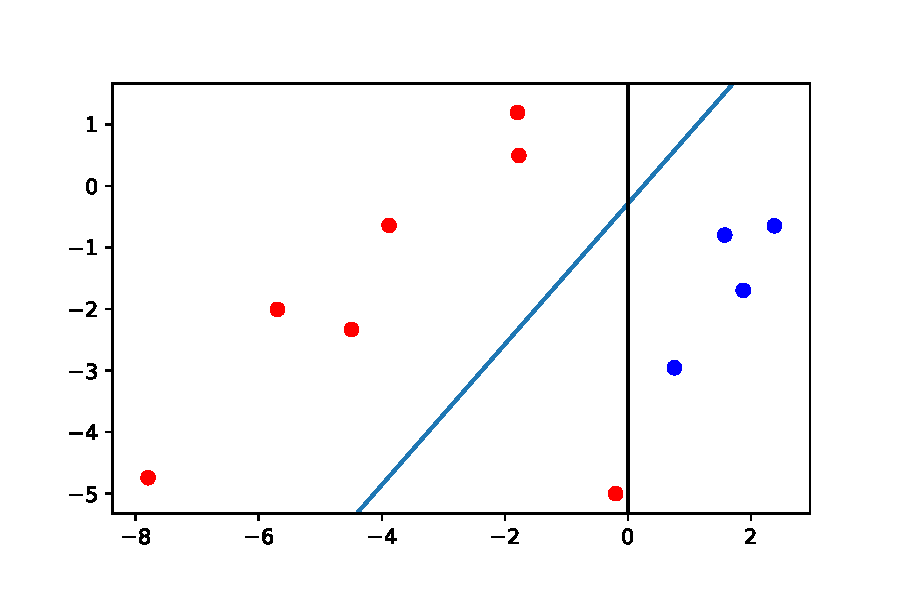
\includegraphics{outlier.pdf}
\caption{Utjecaj stršeće vrijednosti na odabir hiperravnine}
\label{fig:outlier}
\end{figure}

\par Optimizacijski problem je napisan tako da bira razdvajajuću hiperravninu u bilo kojem slučaju, čak i kada
ona nije dobar izbor. Kao rješenje ovog problema uvodi se metoda regularizacije.
\textbf{Regularizacija} je metoda kojom se sprječava pretreniranost modela koristeći funkciju kazne.
Iako je hiperravnina nacrtana crnom bojom na slici \ref{fig:outlier} dobro prilagođena danim primjercima,
kod klasificiranja novih primjerka neće dati dobre rezultate kao hiperravnina označena plavom bojom.
Ovime se kažnjavaju modeli koji pretjerano slijede sve primjerke, ne vodeći računa o generalnoj strukturi 
podataka.

\par Valja navesti dvije najosnovnije funkcije kazne koje se koriste za regularizaciju SVM modela.
Funckija kazne kod L1-SVM modela zadana je izrazom $max(1 - y^{(i)}\mathbf{w}^T\mathbf{x^{(i)}}, 0)$, a
kod L2-SVM funkcija kazne je zadana izrazom $max(1 - y^{(i)}\mathbf{w}^T\mathbf{x^{(i)}}, 0)^2$.
U nastavku će se koristiti L1-SVM.

\par Nakon uvođenja regularizacije, optimizacijski problem može se redefinirati na sljedeći način:
\begin{equation}
\begin{aligned}
& \underset{\mathbf{w}, b}{\text{min}}
& & \frac{1}{2}\|\mathbf{w}\|^2 + C\sum_{i=1}^{N} \xi_i\\
& \text{s obzirom na}
& & y^{(i)}(\mathbf{w}^T\mathbf{x}^{(i)} + b) \geq 1 - \xi_i, \; i = 1, \ldots, N \\
&&& \xi_i \geq 0, \; i = 1, \ldots, N.
\end{aligned}
\label{eq:opt}
\end{equation}

Valja obratiti pažnju na regularizacijski parametar $C$ čiji iznos izražava spremnost na progrešku klasifikaciju
primjerka iz skupa za učenje.
Za velike iznose parametra $C$, optimizacija će inzistirati na ispravnoj klasifikaciji primjeraka iz skupa
za učenje, makar pod cijenu pretreniranosti. Za manje iznose, optimizacija će pogrešno klasificirati 
neke od primjeraka iz skupa za učenje kako bi se pronašla hiperravnina koja dobro opisuje generalnu strukturu
podataka.

\section{Primarni i dualni optimizacijski problem}
Nakon što je optimizacijski problem postavljen, vrijedi ga pokušati i riješiti.
Postupak koji će se koristiti u rješavanju ovog problema je metoda Lagrangeovih multiplikatora.
Neka je zadan \textbf{primarni} optimizacijski problem oblika:
\begin{equation}
\begin{aligned}
& \underset{x}{\text{min}}
& & f(x)\\
& \text{s obzirom na}
& & g_i(x) \leq 0, \; i = 1, \ldots, m \\
&&& h_i(x) = 0, \; i = 1, \ldots, n.
\end{aligned}
\label{eq:lf}
\end{equation}

Za dani optimizacijski problem, može se postaviti Lagrangeova funkcija oblika:
\begin{equation}
\mathcal{L}(x, \alpha, \beta) = f(x) + \sum_{i=1}^{m}\alpha_ig_i(x) + \sum_{i=1}^{n}\beta_ih_i(x)
\end{equation}

gdje su $\alpha$ i $\beta$ Lagrangeovi multiplikatori.
Budući da se traži ekstrem funkcije, Lagrangeova funkcija se parcijalno derivira po varijablama $x, \alpha$
i $\beta$ te se parcijalne derivacije izjednače s nulom. 
Time se dobivaju tri jednadžbe s tri različite nepoznanice.

\par Nakon definiranja Lagrangeove funkcije, valja definirati i još jednu vrijednost:
\begin{equation}
\begin{aligned}
& \theta_\mathcal{P}(x) = \underset{\alpha, \beta, \alpha_i \geq 0}{\text{max}}
& & \mathcal{L}(x, \alpha, \beta).\\
\end{aligned}
\end{equation}

Može se pokazati kako je iznos $\theta_\mathcal{P}(x)$ jednak vrijednosti funkcije $f(x)$ u slučaju kada su svi uvjeti
zadovoljeni. 
U slučaju da neki od uvjeta nisu zadovoljeni, $\theta_\mathcal{P}(x)$ iznosi nula.
Primjerice neka je $g_i(x) > 0$.
Tada se može izabrati $\alpha_i$ za koji desna strana jednadžbe \ref{eq:lf} iznosi $\infty$.
Analogno vrijedi i za $h_i(x) \neq 0$. 
\par Minimizacijom vrijednosti $\theta_\mathcal{P}(x)$ dobije se problem jednak primarnom.
Vrijednost primarnog problema dana je izrazom:
\begin{equation}
\begin{aligned}
& p = \underset{x}{\text{min}}
& & \theta_\mathcal{P}(x).\\
\end{aligned}
\end{equation}

\par Za pronalazak $\theta_\mathcal{P}(x)$ interesantan je bio maksimum Lagrangeove funkcije u odnosu na 
parametre $\alpha$ i $\beta$.
Umjesto toga, problem se može modificrati da umjesto traženja maksimuma u odnosu na parametre $\alpha$ i $\beta$,
traži se minimum u odnosu na $x$. 
\textbf{Dualni} problem definira se na sljedeći način:
\begin{equation}
\underset{\alpha, \beta, \alpha_i \geq 0}{\text{max}} \theta_\mathcal{D}(x) = 
\underset{\alpha, \beta, \alpha_i \geq 0}{\text{max}} \underset{x}{\text{min}} \; \mathcal{L}(x, \alpha, \beta).
\end{equation}

\par Valja primijetiti kako je dualni problem jednak primarnom, uz zamjenu poretka funkcije $min$ i funkcije $max$.
Vrijednost $\theta_\mathcal{D}(x)$ je dana izrazom:

\begin{equation}
\begin{aligned}
& d = \underset{\alpha, \beta, \alpha_i \geq 0}{\text{max}}
& & \theta_\mathcal{D}(x).\\
\end{aligned}
\end{equation}

Uzimajući u obzir odnos između funkcija $max$ i $min$ jasno je da vrijedi relacija $d \leq p$.
No, posebno su interesantni slučajevi gdje su vrijednosti primarnog i dualnog problema jednake.

\par Kako bi vrijednost primarnog i dualnog problema bila jednaka, potrebno je postaviti neka ograničenja
na funkcije $f, g_i$ i $h_i$. Neka je $f$ konveksna funkcija. Nadalje, neka sje $g_i$ konveksne funkcija 
i neka za svaku od njih vrijedi $g_i(x) < 0$. 
Također, neka je $h_i$ linearna funkcija. 
Ako su ti uvjeti zadovoljeni, tada postoje $\alpha, \beta$ i $x$ za koje vrijedi sljedeća jednakost: 
\begin{equation}
  p = d = \mathcal{L}(x, \alpha, \beta).
\end{equation}

Osim gornje jednakosti, za parametre vrijede i Karush-Kuhn-Tucker (KKT) uvjeti:
\begin{equation}
  \frac{\partial \mathcal{L}(x, \alpha, \beta)}{\partial x_i} = 0, \; i = 1, \ldots, p
\end{equation}
\begin{equation}
  \frac{\partial \mathcal{L}(x, \alpha, \beta)}{\partial \beta_i} = 0, \; i = 1, \ldots, n
\end{equation}
\begin{equation}
  \alpha_ig_i(x) = 0, \; i = 1, \ldots, m
  \label{eq:inter}
\end{equation}
\begin{equation}
  g_i(x) \leq 0, \; i = 1, \ldots, m
\end{equation}
\begin{equation}
  \alpha_i \geq 0, \; i = 1, \ldots, m
\end{equation}

Valja napomenuti kako se kod optimizacije stroja s potpornim vektorima u pravilu koristi dualni problem.
Također, za SVM interesantan je uvjet zadan jednakošću \ref{eq:inter}. U pravilu $\alpha_i \neq 0$ iz čega
slijedi $g_i(x) = 0$. Taj uvjet je ključan za pronalazak potpornih vektora.

\section{Optimizacija stroja s potpornim vektorima}
Primjenjujući prethodno poglavlje na optimizacijski problem \ref{eq:opt} primarna Lagrangeova funkcija
može se zapisati
na sljedeći način:
\begin{equation} \label{eq:svmprim}
  \mathcal{L}(\mathbf{w}, b, \xi,\alpha, \mu) = \frac{1}{2}\|\mathbf{w}\|^2 + C\sum_{i=1}^{N} \xi_i
  - \sum_{i=1}^{N} \alpha_i(y^{(i)}(\mathbf{w}^T\mathbf{x^{(i)}} + b) - (1 - \xi_i))
  - \sum_{i=1}^{N} \mu_i\xi_i.
\end{equation}

Vidljivo je kako je ograničenje $y^{(i)}(\mathbf{w}^T\mathbf{x}^{(i)} + b) \geq 1 - \xi_i$ zapisano
kao:
\begin{equation*}
  g_i(\mathbf{w}, b) = - (y^{(i)}(\mathbf{w}^T\mathbf{x^{(i)}} + b) - (1 - \xi_i)) \leq 0.
\end{equation*}

Gore navedeno ograničenje ima zanimljivo svojstvo. 
U slučaju da vrijedi $g_i(\mathbf{w}, b) = 0$ za neki primjerak $(x^{(i)}, y^{(i)})$ tada
taj primjerak se naziva \textbf{potpornim vektorom}. Razumna je pretpostavka kako je potpornih vektora 
relativno malo u odnosu na cijeli skup primjeraka za učenje. Vodeći tom pretpostavkom te uvjetom \ref{eq:inter}
može se zaključiti kako samo za potporne vektore $\alpha_i \neq 0$ dok za ostale primjerke vrijedi 
$\alpha_i = 0$.

\par Primarni problem dan jednadžbom \ref{eq:svmprim} može se derivirati po $\mathbf{w}, b$ i $\xi_i$
i izjednačiti s nulom:
\begin{equation}
  \mathbf{w} = \sum_{i=1}^{N} \alpha_iy^{(i)}x^{(i)}
\end{equation}
\begin{equation} \label{eq:dualcomp}
  0 = \sum_{i=1}^{N} \alpha_iy^{(i)}
\end{equation} 
\begin{equation}
  \alpha_i = C - \mu_i, \forall i.
\end{equation}

Ubacivanjem gornjih jednadžbi u \ref{eq:svmprim}, dolazi se do dualne Lagrangeove funkcije:
\begin{equation} \label{eq:svmdual}
  \mathcal{L}(\alpha) = \sum_{i=1}^{N} \alpha_i - 
  \frac{1}{2}\sum_{i=1}^{N}\sum_{j=1}^{N} \alpha_i\alpha_jy^{(i)}y^{(j)}x^{(i)T}x^{(j)}.
\end{equation}

Uz ograničenje \ref{eq:dualcomp} te ograničenje $0 \leq \alpha_i \leq C$ dualni problem može se zapisati
na sljedeći način:
\begin{equation}
\begin{aligned}
& \underset{\alpha}{\text{max}}
& & \sum_{i=1}^{N} \alpha_i - 
  \frac{1}{2}\sum_{i=1}^{N}\sum_{j=1}^{N} \alpha_i\alpha_jy^{(i)}y^{(j)}x^{(i)T}x^{(j)}\\
& \text{s obzirom na}
& & 0 \leq \alpha_i \leq C, \; i = 1, \ldots, N \\
&&& \sum_{i=1}^{N} \alpha_iy^{(i)} = 0.
\end{aligned}
\end{equation}

Ako se pogleda uvjet \ref{eq:dualcomp} može se zaključiti kako samo potporni vektori utječu na
odabir hiperravnine. U slučaju linearno nerazdvojivih podataka za potporne vektore koji se nalaze
na margini, Lagrangeov multiplikator iznosi $0 < \alpha_i < C$. U slučaju da potporni vektor se ne
nalazi na margini, vrijednost pripadajućeg multiplikatora iznosi $C$.

\section{Jezgreni trikovi} \label{jezgra}
Dosad je optimizacija stroja s potpornim vektorima mogla pronaći razdvajajuću hiperravninu jedino u
slučaju linearno razdvojivih podataka. 
Želja je izgraditi klasifikator koji će moći ispravno klasificirati podatke koji su nisu linearno 
razdvojivi.

\par Kod metoda poput logističke regresije svaki vektor značajki može se, koristeći mapiranje značajki,
preslikati u neki drugi vektor značajki.
Neka je $\mathbf{x}=(x_1, \ldots, x_p)$ vektor značajki. 
Radi jednostavnosti neka postoji samo jedna značajka tj. $\mathbf{x} = (x_1)$.
Neka funkcija $\phi$ vrši polinomijalno mapiranje značajki do trećeg stupnja tj. 
$\phi(x) = (x, x^2, x^3)$. 
Tada vektor značajki $\mathbf{x}$ može se preslikati u 
$\mathbf{x}^{'} = \phi(x_1) = (x_1, x_1^2, x_1^3)$.
Ova ideja može se iskoristiti i kod stroja s potpornim vektorima.
Svaku pojavu vektora značajki $\mathbf{x}$ moguće je zamijeniti funkcijom $\phi(\mathbf{x})$.

\par Valja se na trenutak vratiti na dualnu Lagrengeovu funkciju zadanu jednakošću \ref{eq:svmdual}.
Može se primijetiti kako dio funkcije zadan izrazom $x^{(i)T}x^{(j)}$ je zapravo skalarni umnožak vektora
značajki dvaju primjera. Nadalje će se pisati $\langle x^{(i)},x^{(j)} \rangle$. 
Vektore značajki moguće je preslikati u neke nove vektore značajki koristeći funkciju $\phi$. 
Vrijedi:
\begin{equation*}
  \mathcal{L}(\alpha) = \sum_{i=1}^{N} \alpha_i - 
  \frac{1}{2}\sum_{i=1}^{N}\sum_{j=1}^{N} \alpha_i\alpha_jy^{(i)}y^{(j)}
  \langle \phi(x^{(i)}), \phi(x^{(j)}) \rangle.
\end{equation*}

Primjerak $(x^{(i)}, y^{(i)})$ tada se klasificira na sljedeći način:
\begin{equation*}
  \hat{y} = sgn(\sum_{i=1}^{N} \alpha_iy^{(i)}\langle \phi(x), \phi(x^{(i)}) \rangle
  + b).
\end{equation*}

Vidljivo je kako i dualni problem i funkcija klasifikacije koriste funkciju oblika
$\langle \phi(x), \phi(x') \rangle$, a ne $\phi(x)$. 
Može se definirati \textbf{jezgrena funkcija} oblika:
\begin{equation} \label{eq:trik}
  K(x, x') = \langle \phi(x), \phi(x') \rangle.
\end{equation}

Zamjenu skalarnog umnoška vektora $x$ i $x'$ s jezgrenom funkcijom $K(x, x')$ naziva se
\textbf{jezgreni trik}. 
Najčešće korištene jezgrene funkcije su radijalna bazna funkcija (RBF), polinomijalna i 
sigmoidalna jezgrena funkcija. 
Radijalna bazna funkcija ima oblik:
\begin{equation*}
  K(\mathbf{x}, \mathbf{x}') = \text{exp}(- \frac{\|\mathbf{x} - \mathbf{x}'\|}{2\sigma^2})
\end{equation*}
gdje je $\sigma$ parametar funkcije. Sigmoidalna jezgrena funkcija dana je oblikom:
\begin{equation*}
  K(\mathbf{x}, \mathbf{x}') = \text{tanh}(\gamma\mathbf{x}^T\mathbf{x}' + r)
\end{equation*}
gdje su $\gamma$ i $r$ parametri funkcije.
Polinomijalna jezgrena funkcija zadana je jednadžbom:
\begin{equation*}
  K(\mathbf{x}, \mathbf{x}') = (\mathbf{x}^T\mathbf{x}' + k)^d,
\end{equation*}
gdje je $k$ proizvoljna konstanta, a $d$ stupanj polinoma.
Na primjer, zadan je vektor značajki $\mathbf{x} = (x_1, x_2)$. 
Neka je $k=1$ i $d=2$. Jezgrena funkcija tada iznosi:
\begin{equation*}
  K(\mathbf{x}, \mathbf{x}') = (\mathbf{x}^T\mathbf{x}' + 1)^2 =
  1 + 2x_1x'_1 + 2x_2x'_2 + (x_1x'_1)^2 + (x_2x'_2)^2 + 2x_1x'_1x_2x'_2.
\end{equation*}
Vidljivo je kako smo vektor značajki s dva svojstva mapirali na vektor značajki sa šest svojstava.
Općenito, polinomijalna jezgrena funkcija $d$-tog reda, preslika vektor značajki duljine $p$ u 
vektor značajki duljine $\binom{n + d}{d}$.
Iz povećanja dimenzionalnosti proizlazi i jedan od problema jezgrenih funkcija.
Naime, neka su podaci linearno razdvojivi u slučaju prostora koji sadrži interakcijsku značajku
$x_1x'_1$. Tada je moguće, koristeći gore navedenu polinomijalnu funkciju drugog stupnja, pronaći
razdvajajuću hiperravninu. No, uz ponalazak težine za tu značajku optimizacija traži i težine za ostalih 
pet značajki. Ovaj problem s povećanjem reda jezgrene funkcije postaje sve izraženiji, pogotovo ako je
inicijalni prostor svih primjeraka velike dimenzije.

\section{Višerazredna klasifikacija}
Stroj s potpornim vektorima je binarni klasifikator te sam model nije u mogućnosti klasificirati
primjerke u više od dva razreda.
To ograničenje je intuitivno budući da hipperravnina može razdijeliti prostor u dva potprostora.
Za rješenje ovog problema nude se dvije često korištene metode višerazredne klasifikacije.

\par Prva metoda višerazredne klasifikacije je metoda "jedan-naspram-ostalih" (engl. \textit{one-vs-all}).
Koristeći ovu metodu gradi se sustav klasifikatora.
Ako je zadano $N$ različitih razreda, sustav će biti izgrađen od $N-1$ klasifikatora.
Ovom metodom problem se razbija u više binarnih klasifikacija.
Svaki stroj vrši klasifikaciju za pojedini razred. Vrijednost $1$ označava pripadnost tom razredu dok
vrijednost $-1$ kaže kako primjerak ne pripada razredu.
U slučaju da svih $N-1$ klasifikatora daju negativan izlaz, tada primjerak pripada zadnjem,
$N$-tom razredu. Problem kod ove metode je mogućnost pozitivnog izlaza za više klasifikatora.
Tada sustav nije u mogućnosti odrediti razred kojemu primjerak pripada.

\par Druga metoda višerazredne klasifikacije je metoda "jedan-naspram-jedan" (engl. \textit{one-vs-one}).
Kod ove metode također se gradi sustav klasifikatora, ali kod ove metoda jedan klasifikator vrši usporedbu
između dvaju razreda.
Ukupan broj izgađenih klasifikatora iznosi $\frac{N(N - 1)}{2}$.
Očito je kako je ova metoda vremenski složenija od "jedan-naspram-ostalih" metode. 
No, ova metoda je robusnija u slučaju linearno nerazdvojivih podataka te je robusnija na gore navedeni 
problem jedan-naspram-ostalih" metode.
Sustav radi na principu glasanja. 
Prilikom klasifikacije, svaki klasifikator daje glas nekom od relevantnih razreda. 
Primjerak pripada nekom razredu u slučaju da je taj razred dobio najviše glasova.

\section{Primjena SVM-a kod regresijskih problema}
Stroj s potpornim vektorima je primarno binarni klasifikator. 
No, Drucker je 1997. godine predložio proširenje stroja s potpornim vektorima na 
probleme regresije\cite{Drucker97supportvector}.

\par Neka je zadan linearan model oblika:
\begin{equation}
  f(\mathbf{x}) = \mathbf{w}^T\mathbf{x} + b. 
\end{equation}

Moguće je zapisati funkciju optimizacije na sljedeći način:
\begin{equation}
  f(\mathbf{w}, b) = \sum_{i=1}^{N}L(y^{(i)} - f(\mathbf{x}^{(i)})) + 
  \frac{C}{2}\|\mathbf{w}\|^2
\end{equation}
gdje je $L$ funkcija gubitka, a $C$ regularizacijski parametar. 
Funkciju gubitka $L$ moguće je izabrati na nekoliko načina. 
Neka je $d$ razlika između dane vrijednosti $y^{(i)}$ i vrijednosti izračunate modelom $f(\mathbf{x}^{(i)})$
za neki primjerak $(\mathbf{x}^{(i)}, y^{(i)})$. 
U slučaju da je greška manja od neke proizvoljne vrijednosti $\epsilon$ tada taj primjerak ne pridonosi
ukupnoj grešci. 
U slučaju pogreške veće od $\epsilon$, primjerak pridonosi ukupnoj grešci s $|d| - \epsilon$.
Uspoređujući ovu funkciju gubitka s načinom klasifikacije može se ustvrditi sličnost.
Za primjerke koji su jako udaljeni od hiperravnine klasifikator je veoma siguran da su oni ispravno 
klasificirani te ne utječu na optimizaciju, za razliku od potpornih vektora. 
Kod regresije, primjerci koji su relativno blizu svojoj očekivanoj vrijednosti ne sudjeljuju u funkciji 
gubitka. Može se pisati:

\begin{equation}
  L(d) = 
  \begin{cases}
    0 & \quad |d| < \epsilon\\
    |d| - \epsilon & \quad \text{inače}.\\
  \end{cases}
\end{equation}

Koristeći gore navedene podatke, može se pisati optimizacijski funkcija:
\begin{equation*}
  f(\alpha, \alpha') = \epsilon \sum_{i=1}^{N} (\alpha'_i + \alpha_i) - 
  \sum_{i=1}^{N} y^{(i)}(\alpha'_i - \alpha_i) + \frac{1}{2}\sum_{i=1}^{N}\sum_{j=1}^{N}
(\alpha'_i - \alpha_i)(\alpha'_j - \alpha_j)\langle x^{(i)},x^{(j)} \rangle
\end{equation*}

i pripadajući optimizacijski problem:

\begin{equation}
\begin{aligned}
& \underset{\alpha, \alpha'}{\text{min}}
& & f(\alpha, \alpha')\\
& \text{s obzirom na}
& & \alpha_i \geq 0, \\
&&& \sum_{i=1}^{N} (\alpha'_i - \alpha_i) = 0,\\
&&& \alpha'_i \leq \frac{1}{C},\\
&&& \alpha_i\alpha'_i = 0.
\end{aligned}
\end{equation}

\chapter{Analiza sentimenta} \label{sentiment}

\section{Definicija} \label{def}
Analiza sentimenta (engl. \textit{Sentiment Analysis}) je područje posvećeno 
prikupljanju, obradi i analizi subjektivnih informacija, posebice stavova.
Subjektivne informacije podrazumijevaju kratkoročna stanja poput emocija i raspoloženja,
dugoročna stanja poput stavova pa čak i psihičkih osobina.
S druge strane, objektivne rečenice izriču činjenice. 
Primjerice objektivna rečenica \textit{"Danas je sunčano."} izražava činjenicu te se iz nje ne mogu 
iščitati emocije, stavovi i slično. 
Rečenica poput \textit{"Volim sunčan dan."} govori kako izvor mišljenja ima pozitivan stav prema danima koji
sunčani te je stoga ova subjektiva.
Moguće je da subjektivna rečenica ne izriče stav. 
Rečenica \textit{"Mislim da će sutra biti sunčan dan."} ne predstavlja nikakvu činjenicu, već subjektivni dojam,
no ne izriče nikakav sentiment. 

\par Najčešće promatrana stanja su stavovi pojedinca koji predstavljaju enormni izvor korisnih 
informacija za zainteresirani subjekt.
Koristeći ove informacije, političari mogu osvajati i gubiti izbore, poduzeća plasirati
svoje usluge i proizvode, a potrošći informirati se o istima.
uporabom metoda obrade prirodnog teksta i metoda strojnog učenja, cilj je automatizirati
obradu i analizu subjektivnih informacija.
Upravo subjektivnost čini ovo područje teškim i istovremeno zanimljivim.

\par Problem analize sentimenta može se zadati i na formalniji način.
Neka je dana uređena petorka $(o, k, i, s, v)$ kojom se može definirati sentiment.
Varijabla $o$ predstavlja promatrani objekt. 
Primjerice, ako se analizira kvaliteta mobilnih uređaja, promatrani objekt upravo 
bi bili mobilni uređaji. Varijablom $k$ dana je karakteristika promatranog objekta. 
U slučaju mobilnih uređaja to bi mogla biti kamera, ekran, zvuk, itd.
Ako se analizira uređaj u cjelini, tada ova varijabla može biti zanemarena.
Varijabla $i$ predstavlja izvor mišljenja, korisnika.
Ključni dio problema, sentiment, dan je varijablom $s$. 
Sentiment predstavlja mišljenje korisnika $i$ o nekoj karakteristici $k$ proizvoda $o$.
Mišljenja, stavovi i emocije mijenjaju se s vremenom pa je važno uključiti i vrijeme u sam
problem. 
Vrijeme je predstavljeno varijablom $v$.

\par Evo i jednog primjera korisničke recenzije operacijskog sutava
\footnote{Napomena: Iako nije dano ime operacijskog sustava, čitatelj može s jednostavnošću
zaključiti o kojem se operacijskom sustavu radi}: \\
{\it
Užasan operacijski sustav. 
Osim osnovnih alata, upakiran je i s gomilu programa koji samo usporavaju rad sustava.
Nadam se da korisnici nisu ljubitelji privatnosti jer ju s ovim operacijskim sustavom
sigurno neće imati. 
Jedina pozitivna opcija je uvođenje radnih sati tako da me sustav rjeđe maltretira s 
ponovnim pokretanjem.
Savjet: potražite alternativu.
} Marko, 2016.
\par Nakon čitanja korisničke recenzije, jasno je kako se ovdje radi o negativnoj recenziji
proizvoda.
Prva rečenica recenzije je najbitnija za određivanje sentimenta prema cijelom proizvodu.
Izvor mišljenja, korisnik Marko, ocjenjuje cijeli sustav \textit{užasnim}.
Izbor pridjeva, u ovom slučaju \textit{užasan}, sigurno utječe na intenzitet sentimenta. 
Kad bi se umjesto navedenog pridjeva našao pridjev \textit{loš} i dalje bi izjava bila
klasificirana kao negativna, no s puno manjim intenzitetom u odnosu na izjavu koja sadrži pridjev 
\textit{užasan}.
Nakon prve rečenice, slijede dvije rečenice negativnog sentimenta usmjerene na pojedine karakteristike
sustava. Četvrta rečenica navodi jednu pozitivnu karakteristiku sustava.
U slučaju analize sentimenta na razini cijele recenzije ova rečenica uvodi šum te predstavlja jedan od
problema u analizi sentimenta. 
Iz zadnje rečenice, iako svakako manjeg intenziteta od ostalih, također se može iščitati negativan 
stav prema proizvodu. Valja napomenuti kako je ova recenzija napisana 2016. godine te upravo godina 
predstavlja vremensku komponentu problema. Moguće je da se s vremenom stav korisnika promijeni.
Tada ova recenzija više neće biti aktualna. Ukupno se može iščitati četiri sentimenta: 
\begin{center}
(Operacijski sustav, "općenito", Marko, negativan, 2016.)\\
(Operacijski sustav, programski paket, Marko, negativan, 2016.)\\
(Operacijski sustav, razina privatnosti, Marko, negativan, 2016.)\\
(Operacijski sustav, vrijeme osvježavanja sustava, Marko, pozitivan, 2016.) \\
\end{center}

\section{Tipovi mišljenja} \label{samisljenje}


\section{Razine analize sentimenta} \label{sarazine}
Sentiment korisnika može se proučavati na više razina.
U pravilu sentiment korisnika proučava se na sljedeće tri razine:

\begin{enumerate}
  \item \textbf{Analiza na razini dokumenta}. 
  Cilj ove razine je pronaći generalni sentiment u sklopu cijelog teksta. 
  Provodi se najćešće kada zainteresirane strane ne zanima sentiment neke karakteristike proizvoda
  ili usluge već generalan stav.
  Također, pretpostavlja se da korisnik ocjenjuje samo jedan proizvod budući da iz njega nije moguće
  iščitati mišljenje o više proizvoda.
  Primjer analize na razini dokumenta je analiza korisničkih recenzija filmova 
  \cite{Pang+Lee+Vaithyanathan:02a}.

  \item \textbf{Analiza na razini rečenica}.
  Cilj analize na razini rečenica je odrediti pozitivnost, neutralnost ili negativnost svake rečenice.
  Za ovu razinu analize važno je razlikovati objektivne i subjektivne rečenice 
  \cite{wiebe-bruce-o'hara:1999:ACL}.
  No, postoje iznimke kada rečenice, iako objektivne, nose sentiment.
  Primjerice, \textit{"Capacitet baterije ovoga mobitela drastično opada već nakon dva mjeseca."}
  predstavlja objektivnu rečenicu, ali i implicitno izlaže nezadovoljstvo korisnika.

  \item \textbf{Analiza na razini karakteristika}.
  Najdetaljnija i najkompleksnija analiza sentimenta vrši se na razini karakteristika.
  Pretpostavka je da svako mišljenje sadrži sentiment i objekt te da mišljenje nije striktno vezano
  uz formu tj. uz rečenicu, paragraf, cijeli dokument \cite{Hu:2004:MSC:1014052.1014073}.
  Na primjer, rečenica \textit{"Zadovoljan sam s mobitelom marke A, no nije kao onaj marke B."}
  izražava pozitivan stav prema oba mobitela, no intenzitet sentimenta nije jednak prema oba mobitela.
  Viljivo je kako postoji dva sentimenta i dva različita objekta što se ne može utvrditi na razini rečenice,
  a pogotovo na razini dokumenta.
  Rečenica \textit{"Auto je brz, ali troši previše goriva."} izražava sentiment o jednom objektu, autu, 
  ali za više njegovih karakteristika.
  Upravo je pronalazak karakteristika i objekata veoma složen problem koji čini ovu razinu još kompleksnijom
  u odnosu na razine dokumenta i rečenice. 
\end{enumerate}

Iako su sve tri razine analize sentimenta zanimljive i složene, u ovom radu fokus je stavljen na 
razinu dokumenta.

\section{Sentiment na razini dokumenta} \label{sadoc}

\section{Problemi kod analize sentimenta} \label{saprob}

\chapter{Implementacija i rezultati} \label{eksperiment}

\chapter{Zaključak} \label{zakljucak}
Zaključak.

\bibliography{literatura}
\bibliographystyle{fer}

\begin{sazetak}
Sažetak na hrvatskom jeziku.

\kljucnerijeci{Ključne riječi, odvojene zarezima.}
\end{sazetak}

% TODO: Navedite naslov na engleskom jeziku.
\engtitle{Application of Support Vector Machine for Users' Reviews Sentiment Analysis}
\begin{abstract}
Abstract.

\keywords{Keywords.}
\end{abstract}

\end{document}
